\section{Packet streaming}\label{sec:terminologies}

To fairly compare different data reduction techniques is challenging. One popular method is to
restrict the techniques to the same data size, and compare data quality. It is however difficult to
enforce, for example, that a multi-resolution scheme uses the same amount of data as a quantization
scheme does. This is because going down one step in resolution decreases the data size by a
different amount from removing one more bit from each data sample. To avoid this mismatch of data
increment/decrement units, we model each reduction scheme as a stream of equal-size \emph{packets}.
A packet forms the smallest unit of data increment/decrement in our framework, and each consists of
a relatively small number of bits from a data set. To study the resolution-versus-precision
tradeoffs, we associate a packet with a resolution level and a precision level (i.e., bit plane), so
that each packet can improve either data's resolution or precision. In this framework, different
data reduction schemes become different orderings of packets from a data set, or different packet
\emph{streams}. For example, a quantization scheme would stream packets by precision, while a
multi-resolution scheme would stream packets by resolution. By forcing the different schemes to use
the same number of packets, we can compare data quality across the schemes more fairly.

In \autoref{sec:data-streaming-framework} we discuss the mechanism of converting original data into
a set of packets. \autoref{sec:static-dynamic-streams} is about packet streams that correspond to
common data reduction schemes. \autoref{sec:data_dep_streams} presents a greedy algorithm to
approximate the optimal packet stream for the data and the analysis task at hand. Finally,
\autoref{sec:stream-signature} introduces a novel concept called \emph{stream signature} that can be
used to study and compare the characteristics of different packet streams.

\subsection{Decomposition of data into packets}\label{sec:data-streaming-framework}
Each packet is supposed to improve data's resolution and/or precision. To introduce the concept of
resolution, we use the popular CDF5/3 discrete wavelet transform [CITE]. Although there exists other
transforms that separates a signal into discrete bands of frequencies/scales/resolutions, such that
the discrete Fourier transform, we choose wavelet because wavelet coefficients are spatially
localized. This enables spatial adaptivity, allowing finer resolution in regions containing
important features, at the expense of coarser resolution elsewhere. The hierarchical-Z indexing
scheme [CITE] also produces a multi-resolution representation, but unlike wavelet, it offers no
interpolation mechanism for low-resolution grids. The CDF5/3 wavelet is chosen for its balance
between simplicity and effectiveness at decorrelating the input signal. It is also one of the two
transforms of choice in the JPEG2000 standard [CITE].

The typical multi-dimensional wavelet transform can be performed in multiple passes, which
eventually results in the original domain being partitioned into several \emph{subbands}, each can
be thought of as a resolution level. One transform pass creates four subbands in 2D, and eight in
3D, of which the first is a smoothed, downsampled version of the original data. The next seven
subbands (in 3D) add fine details in each subset of the dimensions. A subsequent transform pass
typically recurs on the first subband created by the previous pass, leaving the other seven subbands
intact. We frequently use $l$ to index the subbands, which starts from 0 (referring to the coarsest
subband), and use $L$ to denote the highest-indexed subband. In this paper, $L=21$ (in 3D),
corresponding to three passes of transform.

For precision, we quantize floating-point wavelet coefficients to $B$-bit signed integers. For most
of the experiments in this paper, $B=16$. This quantization eliminates the exponent bits, so that
every bit (except the sign bit) can be associated with a bit plane $b$ ($0\leq b\leq B-1$),
contributing $2^b$ in absolute value to its coefficient's value. To further avoid treating the sign
bit specially, we convert quantized coefficients from two's complement form to negabinary form, in
which integers are represented in base negative two (i.e., $\sum_{i=0}^{B}{c_i(-2)^i}$ with $c_i\in
\{0,1\}$). This transformation increases the number of bit planes by one, to compensate for the
absence of the sign bit. We use $b$, which starts from 0, to index the bit planes, with the
convention that higher-indexed bit planes are less significant.

As mentioned earlier, in our framework, the smallest unit of data is called a \emph{packet}.
Precisely, a packet consists of bits on the same bit plane, from a \emph{block} of negabinary
wavelet coefficients. A block is a $g\times g\times g$ grid of adjacent coefficients on the same
subband. We let $g$ be a constant, so that finer-resolution subbands contain more packets. This
enables the natural tradeoff between wider (but coarser) coverage and finer (but more local)
details, for the same number of packets. In this paper, a packet always contains $4096$ bits (i.e.,
$g=16$), following the common practice of reading bits in batch for performance reason. This choice
of $g$ also accelarates our experiments significantly, without affecting the results in a meaningful
way.

A data reduction scheme can be modeled as an ``inverse'' stream of packets, where the original data
contains all packets, and any reduction step removes certain packets based on some criteria (more
details in \autoref{sec:static-dynamic-streams}). In our data streaming model, there is a ``server''
which serves data and a ``client'' which receives data from the server. At any point, the client is
assumed to have received a subset of packets from the server, which it can use to reconstruct the
original function (using the inverse wavelet transform). Therefore, to compare different streams, we
can reconstruct the original data using the same number of packets from each, and perform analysis
tasks on each of the (approximate) reconstructions. A stream is better suited for an anlysis task if
it produces results that are closer to reference results computed from the original data.
\autoref{fig:pipeline} gives a schematic view of our data streaming model.

\begin{figure}[h]
  \centering
  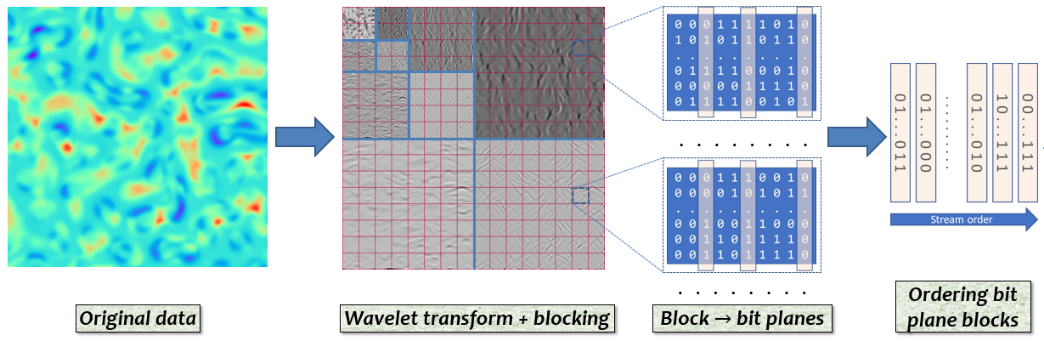
\includegraphics[width=\linewidth]{img/pipeline.png}
  \caption{Our data streaming model (in 2D). The input is a regular grid of floating-point samples,
  the output is a stream of packets. Different data reduction schemes generate different streams.
  The wavelet subbands are separated by blue lines in the second image, with the coarsest subband at
  the top left corner. Although not showed here, quantization and negabinary convesion happen
  immediately after wavelet transform. TODO: revise this figure}\label{fig:pipeline}
\end{figure}

\subsection{Data-dependent and data-independent streams}\label{sec:static-dynamic-streams}

While both the server and the client in our model can be on the same physical machine, only the
server has full knowledge of the data. Thus, when the client receives a packet, it might not know
where that packet should be deposited. A common solution is to have both the client and the server
agree beforehand on a static ordering of packets, independent of the data. We use the term
\emph{data-independent streams} to refer to streams using this solution. In constrast, for
\emph{data-dependent streams}, the client is assumed to ``magically'' know the positions of packets
without receiving this information from the server.

A stream can be viewed a collection of packets, sorted in descending order of some weight associated
with each packet $p$. Two sorting criteria, corresponding to two common data reduction schemes in
the literature, are \emph{by level} and \emph{by bit plane}. The \emph{by level} stream orders the
packets strictly from coarser to finer resolution levels. The weight function in this case is
$W_{lvl}(p)=L-l(p)$, where $l(p)$ is the subband index of $p$, and $L$ is the total number of
subbands. Within the same subband, without any assumption on the underlying data, packets follow the
row-major order of coefficients, then bit plane order (from 0 to $B$) within each coefficient. The
other common ordering, \emph{by bit plane}, proceeds strictly from higher-ordered to lower-ordered
bit planes. That is, $W_{bit}(p)=B-b(p)$, where $b(p)$ is the bit plane index of $p$, and $B$ is the
total number of bit planes. Within the same bit plane, packets follow the subband order (from 0 to
$L$), then row-major order in each subband. We use $s_{lvl}$ and $s_{bit}$ to denote the \emph{by
level} and the \emph{by bit plane} streams.

$s_{lvl}$ and $s_{bit}$ are designed to mimic the way data is accessed in traditional methods that
work either in resolution ($s_{lvl}$) or in precision ($s_{bit}$). We also define a third stream,
called \emph{by wavelet norm} and denoted as $s_{wav}$, which combines these two dimensions.
$s_{wav}$ orders packets using $W_{wav}(p)=2^{B-1-b(p)}\times \norm{\omega_{l(p)}}^2$. The first
term captures the contribution of a bit on bit plane $b(p)$, while the second term captures the
contribution of a wavelet coefficient on subband $l(p)$, where $\omega_{l(p)}$ refers to a wavelet
basis function on subband $l(p)$. In the wavelet representation, a function $f$ is written as a
linear sum of wavelet basis functions $\omega_i$: $f=\sum{c_i\omega_i}$, where $c_i$ are the
coefficients. Since basis functions in the same subband share the same norm, $W_{wav}(p)$ is simply
the contribution (in $L_2$ norm) of a bit on bit plane $b_p$ and subband $l_p$, to the whole
function $f$. To our knowledge, a data reduction scheme based on \emph{by wavelet norm} was hinted
at in [CITE]. \duong{if there is enough space, include here the formula to compute the norm of basis
functions, else put it in the appendix}

Another data common reduction technique, especially for transform-based data, is one in which
truncation happens by by leaving out coefficients of smallest magnitudes. We model this scheme with
a stream called \emph{by magnitude}. Here, the weight function is $W_{mag}(p)=\sum_{c\in
block(p)}\norm{c}^2$ (the sum is over all coefficients in the block that contains packet $p$). If
two packets have the same weight, they are ordered by subband index, then by bit plane. Unlike
\emph{by level} and \emph{by bit plane}, \emph{by magnitude} is data-dependent, because the
coefficient magnitudes are not known until after the data has gone through the wavelet transform. We
use $s_{mag}$ to denote this stream.

In general, data-dependent streams are better than data-independent streams in theory, because they
can prioritize important packets based on the actual data. However, data-dependent streams are
ill-suited for practical purposes, because the cost of sending position information likely
outweights any potential benefit. Despite that, we study them for various reasons. First, the
\emph{by magnitude} scheme is well-known in the literature. Second, data-dependent streams can serve
as a benchmark to evaluate the performance of their data-independent counterparts. Finally, in
addition to being data-dependent, streams can also be task-dependent
(\autoref{sec:data_dep_streams}), which may provide insights on how data should be queried to
perform certain analysis tasks.

\subsection{Constructing data-dependent, task-optimized streams}\label{sec:data_dep_streams}
Each analysis task potentially requires a fundamentally different stream for optimal results. Two
streams can be compared on the basis of how well they work for an analysis task, provided that an
error metric for that task is well defined. This section aims to solve the problem of finding the
optimal (and data-dependent) stream, given a data set and such an error metric. Studying such as
stream is important because it serves not only as a benchmark, but also as a source of insights for
other, more practical streams for the same task.

An error metric is a function $e(q(f'),q(f))$ that returns the distance between its two arguments.
$f$ is the original data and $f'$ is a reconstructed version of $f$ using a subset of the packets.
$q$ is some quantity of interest (e.g., histogram, isocontour, etc) derived from $f$ or $f'$. In
this paper we use the terms ``quantity of interest'' and ``task'' interchangebly, with the
understanding that if the task is extracting an isocontour, then the quantity of interest is an
isocontour. For each task $q$, we choose one error metric $e$ that is either common, or intuitive
and simple while generalizable. Given a data set $f$, a task $q$, and an error metric $e$, we aim to
generate a stream $s_{opt}$ that is optimal for $q$ in terms of $e$.

One way to define the ``optimal'' stream could be one that incurs the minimum error $e$ at every
point. In trying to realize it, however, our experience has been that such a stream does not exist.
Assume otherwise that the optimal stream exists, then by definition, it must be possible to
construct this stream (called $s_{opt}$) using the following greedy algorithm. Start with a pool
consisting of all packets, an all-zero function $f'$, and an empty $s_{opt}$. From the pool, pick
one packet $p$ that when applied to the current $f'$, would minimize $e$. Remove $p$ from the pool,
add it to the end of $s_{opt}$, and update $f'$ using $p$. Repeat this process until the pool is
empty. This algorithm can encounter a situation in which the chosen packet $p$ contributes almost
nothing to $f'$, yet the error is minimized because it is kept approximately constant. In this case,
it is actually better to pick another packet that increases the error slightly, but otherwise
contributes a lot more to $f'$. In optimization terms, it is necessary to follow a search direction
that increases the error slightly to avoid being stuck in a local minimum. This contradiction shows
that $s_{opt}$ does not exist, using the aforementioned definition of optimality.

We can change the definition of $s_{opt}$ to be a stream such that the area bounded by its error
curve (when plotted) and the horizontal axis is the smallest. However, this definition is of limited
usefulness in practice, because a stream should be able to terminate at any point, and still
produces an error as small as possible. Therefore, instead of using this definition of optimality,
we slightly modify the greedy algorithm above to avoid local minima. We still start with a pool
consisting of all packets and an empty $s_{opt}$, but with a ``lossless'' $f'$ (i.e., $f'=f$), and
we build $s_{opt}$ back-to-front. In each step, the packet whose removal from $f'$ has the least
impact on the error $e$ is removed from both $f'$ and the pool, and inserted to the beginning of
$s_{opt}$. This algorithm solves the previous problem where unimportant packets were added to
$s_{opt}$ too early (i.e., the algorithm gets stuck in a local minimum). Here, packets chosen early
are actually unimportant, and will be put at the end of $s_{opt}$.

Unfortunately, we have found that this back-to-front greedy algorithm is too costly in practice.
Ignoring all the steps done in each iteration, this algorithm amounts to a 2-level nested loop
running for $n^2$ iterations, where $n$ is the total number of packets. With a $256^3$-size domain,
a packet size that spans $16^3$ coefficients, and $16$ bits of quantization, $n$ is 65536, so $n^2$
would be in the billions, which we have found to be prohibitively large. We have therefore adopted a
simplified version of this algorithm, where only one pass through the set of $n$ packets is needed.
The modified algorithm works as follows. In each iteration $i$, we disable (set to zero) a new
packet $p_i$ in $f'$, then compute and record the incurred error $e_i$. $p_i$ is enabled again in
$f'$ at the end of iteration $i$. After $n$ iterations, each packet has an associated weight $e_i$.
$s_{opt}$, then, is simply the sorted list of packets in decreasing order of the weights. This
simplified algorithm brings the running time from days down to minutes, while (by observation)
retaining the same quality for $s_{opt}$. The pseudocode of the algorithm is presented in
Algorithm~\autoref{alg:greedy}.

\begin{algorithm}[h]
  \small
  %\algsetup{linenosize=\small}
  \caption{Computing a task-optimized stream}
  \begin{algorithmic}[1]
    \Inputs{
			An original function $f$\\
			An unordered set of $n$ packets $P = \{p_i\}$, produced from $f$\\
			A quantity of interest $q$, and an error function $e$}
		\Initialize{A set of $n$ weights $\Gamma = \{\gamma_i\}$ }
		\For{each packet $p_i$}
			\State $p_i := 0$
      \State $P \rightarrow$ wavelet coefficients $W$ (inverse quantization and inverse negabinary transform)
			\State $W \rightarrow f'$ (inverse wavelet transform)
			\State $\gamma_i := e(q(f'),q(f))$			
			\State Restore $p_i$
		\EndFor
		\State Sort the $p_i$'s in descending order of $\gamma_i$.
		\Output{The $q$-optimized stream, which is the sorted $P$}
	\end{algorithmic}
	\label{alg:greedy}
\end{algorithm}

\subsection{Stream signatures}\label{sec:stream-signature}

Denote the 2D space of bit planes versus subbands (or precision versus resolution) as $S_{L,B}$
(i.e., $S_{L,B}=\{(l,b) | 0\leq l\leq L, 0\leq b\leq B\}$). Unlike data-independent streams,
data-dependent streams do not impose a static ordering of packets in this space. Therefore, to
analyze this aspect of a data-dependent stream, we introduce the concept of a \emph{stream
signature}. Given a stream, a signature $A_{L,B}$ is an $L \times B$ matrix, whose $(l,b)$ element
is associated with $P_{l,b}$ --- the set of packets belonging to subband $l$ and bit plane $b$. In
particular, $A(l,b)$ is an integer in the $[0, B\times L)$ range that indicates, on average, the
position in which $P_{l,b}$ appear in the given stream. For example, the signature $A=\bigl[
\begin{smallmatrix}0 & 1 & 4\\ 2 & 3 & 5\end{smallmatrix}\bigr]$ indicates that the stream begins
with packets that lie on the first bit plane of the first subband, as $A(0,0)=0$. Those are followed
by packets on the second bit plane of the first subband ($A(0,1)=1$), then the first bit plane of
the second subband ($A(1,0)=2$). Finally, the last group of packets comes from the third bit plane
of the second subband ($A(1,2)=5$). A stream's signature shows how the stream traverses the space
$S_{L,B}$. In this way, the signature concept can reveal the potentially different
resolution-versus-precision tradeoffs among $s_{opt}$ streams optimized for different tasks.

To compute a stream signature, we partition the whole domain (not individual subbands) into several
\emph{regions}, compute one signature per region, then average over these local signatures. It is
only when packets are relatively well localized, that their relative ordering in the $S_{L,B}$ space
becomes meaningful. For example, a packet at one corner of the domain can be streamed before one at
an opposite corner, but this fact contains no useful information. We define a region to be the
spatial volume that is covered by a packet in the coarsest subband. Algorithm~\ref{alg:signature}
lists the steps in detail.

\begin{algorithm}[h]
  \small
  \caption{Computing a stream signature}
  \begin{algorithmic}[1]
    \Inputs{
			A stream $P=\{p_i\}$\\}
		\Initialize{Per-region signature matrix $A_r:= 0$\\
		Global signature matrix $A := 0$}
		\For{each packet $p_i$ in $P$}
			\State Let $r$, $b$, $l$ be the region, bit plane, and subband that $p_i$ belongs
			\State $A_r(l,b) := A_r(l,b)+i$
		\EndFor
		\For{each region $r$}
			\State Sort the elements of $A_r$
			\State Assign each element of $A_r$ its index after sorting
			\State $A := A+A_r$
		\EndFor
		\State Sort the elements of $A$
		\State Assign each element of $A$ its index after sorting
		\Output{The signature matrix $A$}
	\end{algorithmic}
	\label{alg:signature}
\end{algorithm}

Finally, a signature can be used to construct a ``semi'' data-independent stream, denoted as
$s_{sig}$. This is done by iterating through each element $A(l,b)$ in ascending order, and adding
end of $s_{sig}$ all the packets in $P_{l,b}$. $s_{sig}$ is similar to purely data-independent
streams, in that the ordering of packets in the $S_{l,b}$ space is deterministic (governed by the
signature). However, this deterministic ordering must be established between the client and the
server through the transmission of the signature. This is not a hurdle in practice, because the size
of the signature should be negligible compared to the size of the data itself. In 3D, assuming 22
subbands and 32-bit quantized coefficients, a signature contains $1408 (=22\times 32\times 2)$
bytes. $s_{sig}$ has no element of spatial-adaptivity, hence it can serve as a bridge when comparing
the resolution-versus-precision tradeoffs between data-independent and data-dependent streams.
